\section{Results}
\label{Resul}

The following Section summarises the work by presenting the obtained results. Comments on the goodness of such results are also present, together with possible future developments. 
The popularity distribution computed through Eq. (\ref{Popc}) shows a gaussian-like distribution centred in 0 (Fig. \ref{PopDist}), meaning that on average comments are neutral, with lateral tails of comments with strong polarity, both positive and negative. Recommendations play a small role, because of some outliers causing the normalised recommendation count to be quite a small number. It is fundamental for this distribution to be unbiased as it will be used to estimate controversy in different articles. 

\begin{figure}
\centering
    \begin{subfigure}{0.5\tw}
    \centering
    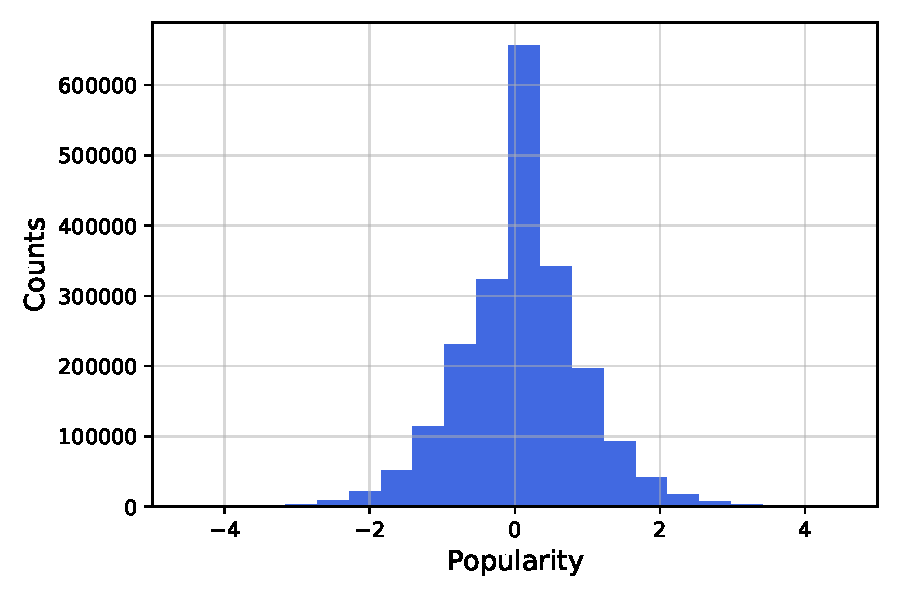
\includegraphics[height=4cm]{Pictures/PopularityDist.pdf}
    \caption{Popularity distribution}
    \label{PopDist}
    \end{subfigure}%
\hfill
    \begin{subfigure}{0.5\tw}
    \centering
    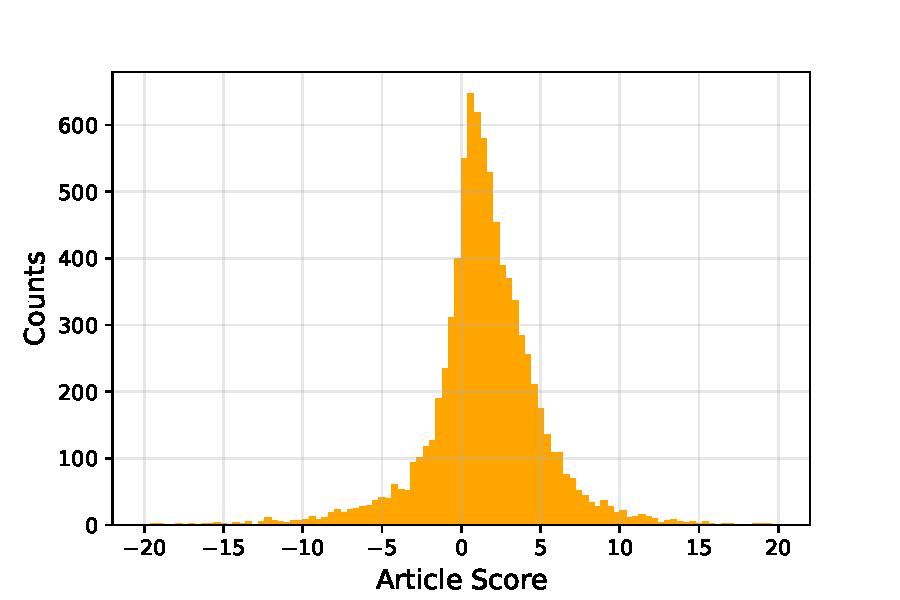
\includegraphics[height=4.5cm]{Pictures/articleScoreDist.pdf}
    \caption{Article score distribution.}
    \label{AScore}
    \end{subfigure}
\caption{Preliminary distributions.}
\end{figure}

The article score distribution shows a similar behaviour; it is reported in Fig. \ref{AScore} even though it will not be included in further analyses. Again, the article Score calculated with Eq. \ref{ASeq} shows a quite symmetrical distribution, meaning that the estimator is consistent and the articles are distributed equally among the polarity spectrum.

\subsection{Strategy 1 (linear)}
\label{Strategy1}
The first strategy to estimate controversy in news articles (Eq. \ref{Str1}) was to multiply the number of comments related to each article with the IQR of the popularity distribution for such comments (labelled as \textit{debate}). This calculation lead to an index of controversy peaked near 0. Furthermore, the controversy distribution looks very similar to the comment number distribution (see Fig. \ref{Str1Dist}). This suggests that popularity and controversy are strongly correlated, while debate plays an insignificant role in the compute. 

\begin{figure}[tb]
\centering
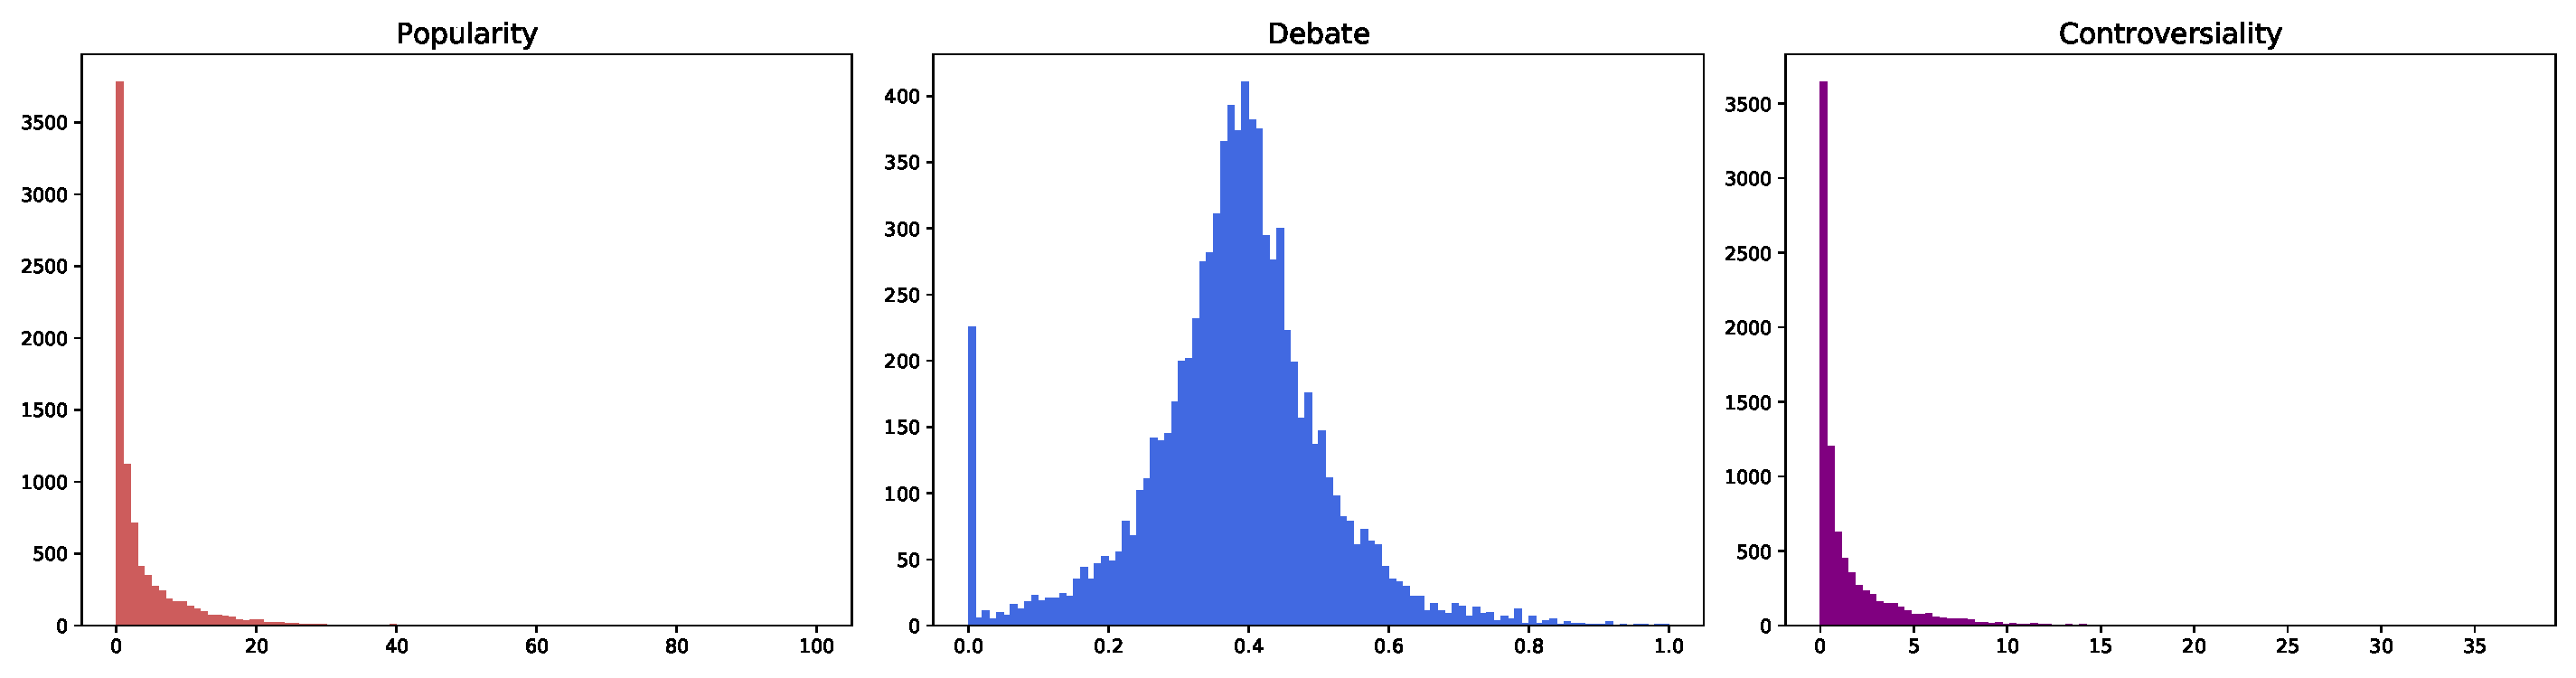
\includegraphics[width=\tw]{Pictures/Strat1Dist.pdf}
\caption{Popularity, Debate and Controversy distributions for Strategy 1}
\label{Str1Dist}
\end{figure}

To corroborate this hypothesis, the correlation scatter plots for the three variables were built, and Fig. \ref{Str1Corr} shows a very strong linear correlation between popularity and controversy. This correlation rows against the thesis of the project, which is trying to differentiate the so-called "hot topics" from the most controversial ones. For this reason, another strategy was implemented to see if some other definition of controversy can detach more efficiently from the concept of popularity.

\begin{figure}[tb]
\centering
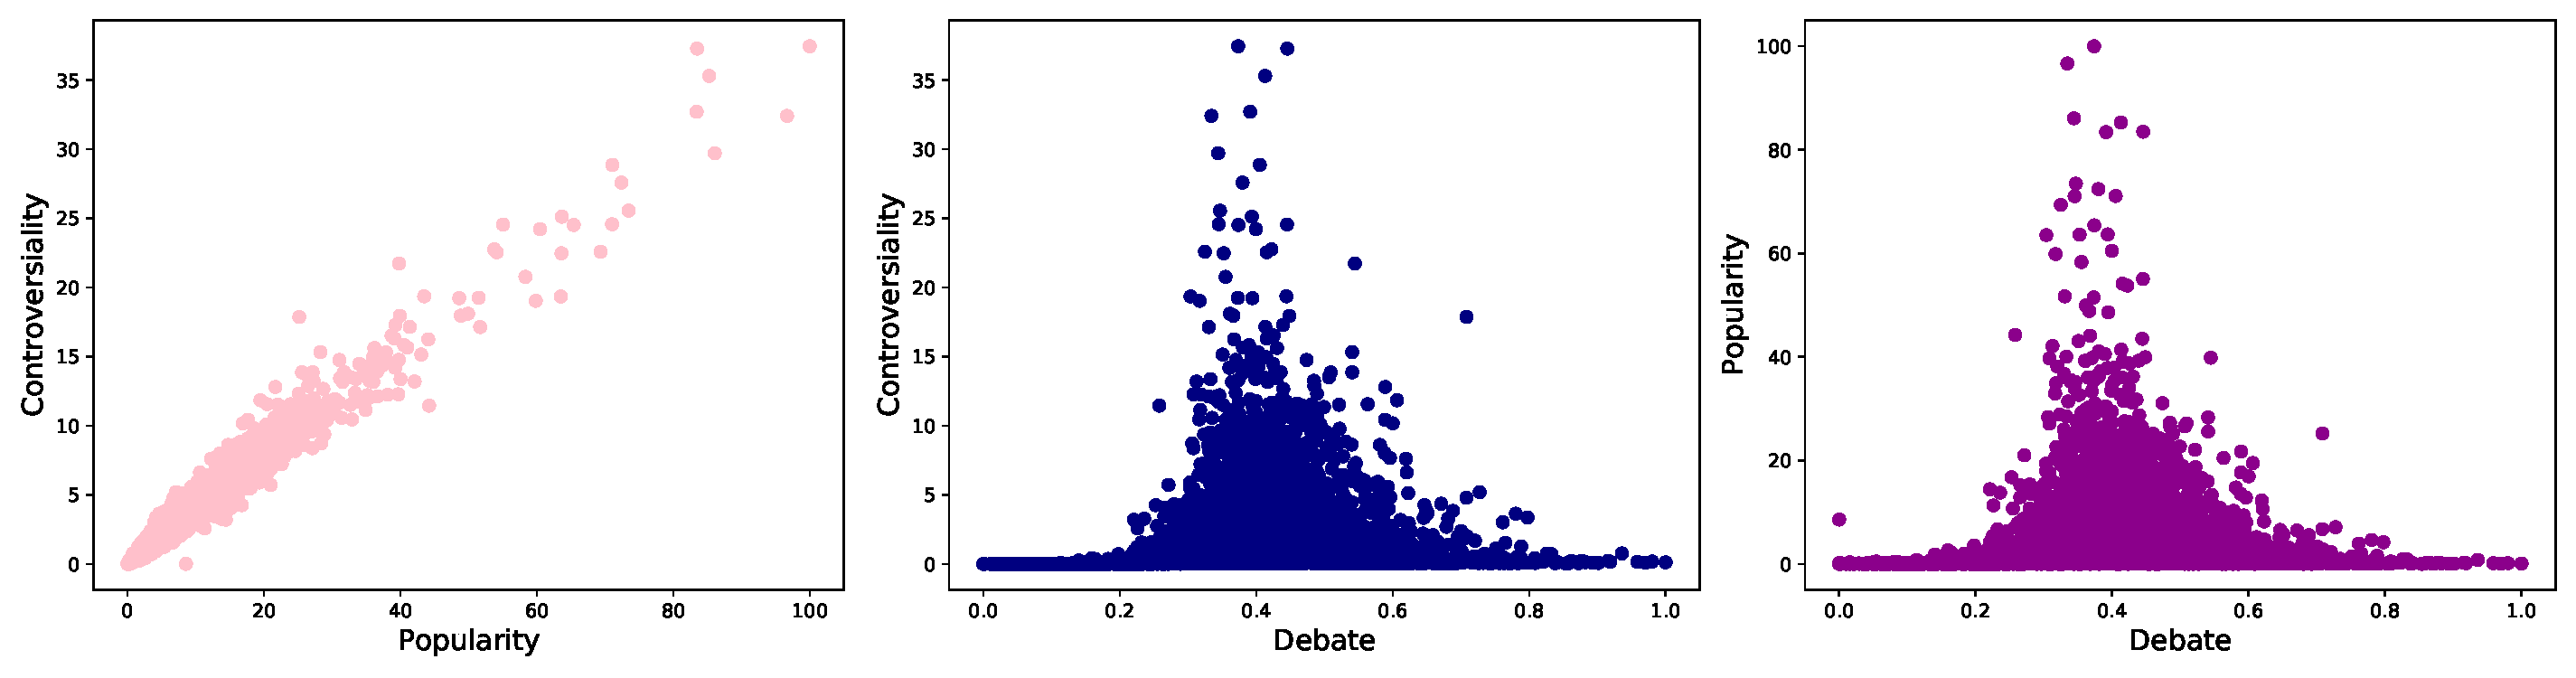
\includegraphics[width=\tw]{Pictures/Strat1Corr.pdf}
\caption{Correlation plots for Strategy 1.}
\label{Str1Corr}
\end{figure}

To go deeper into the analysis, the controversy scores for each articles were averaged among articles of the same section. This grouping was made to see if any article section is more controversial than others. Unfortunately, Strategy 1 did not prove to be useful in this case, as the most controversial topics are also the most popular one. Figure \ref{RG1} shows how, for each section, the controversy and the popularity score look very similar to each other (after proper normalisation).

\begin{figure}
\centering
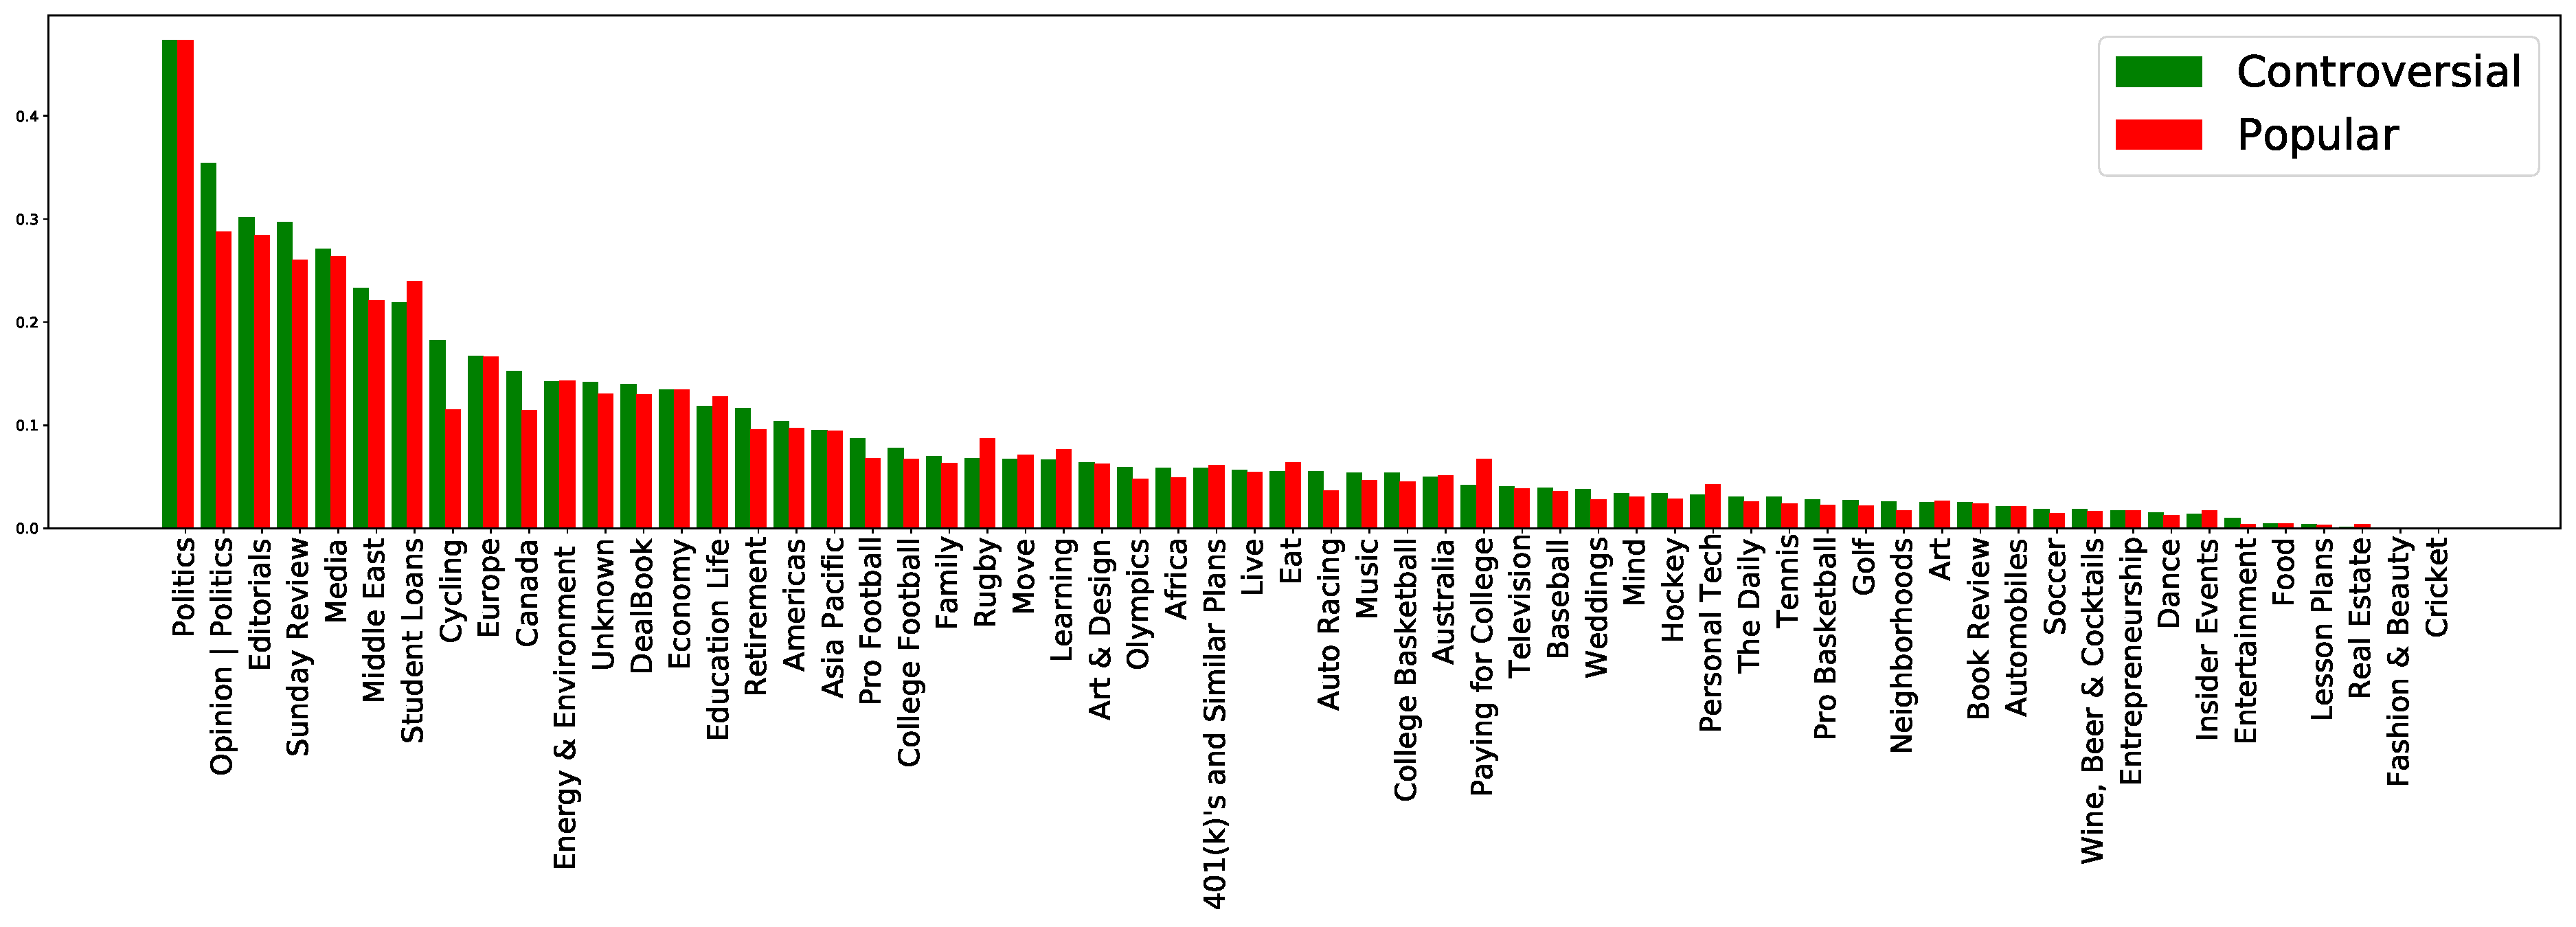
\includegraphics[width=\tw]{Pictures/Strat1SN.pdf}
\caption{Most controversial sections for Strategy 1}
\label{RG1}
\end{figure}

After that, articles were also grouped by the "new desk" index, to see if there is any category that stands out as the most controversial. Again, results (Fig. \ref{RG1nd}) indicate a high similarity between controversy and popularity, with "National" desk as the most popular desk.

\begin{figure}
\centering
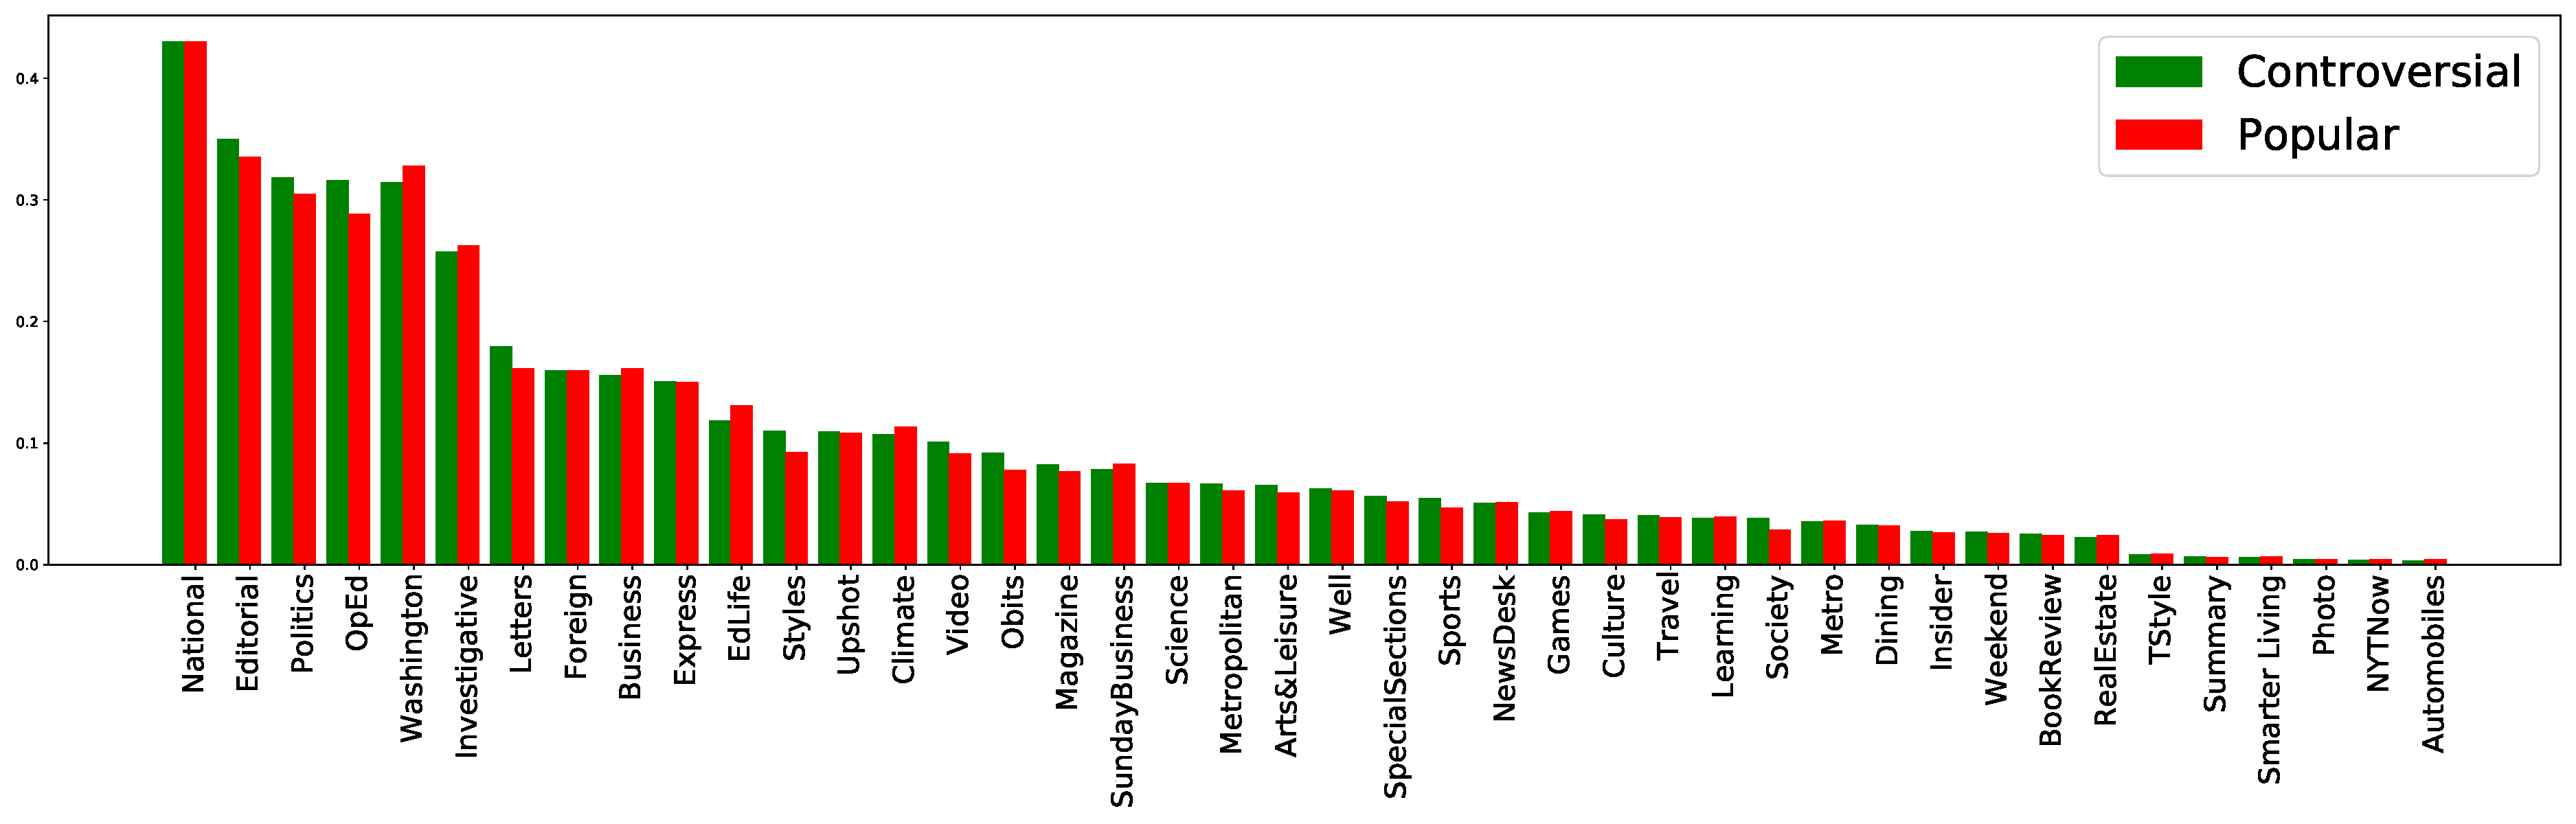
\includegraphics[width=\tw]{Pictures/Strat1ND.pdf}
\caption{Most controversial desks for Strategy 1}
\label{RG1nd}
\end{figure}

\subsection{Strategy 2 (log)}

Strategy 2 consisted on applying the natural logarithm to the number of comments under each article, in order to dampen the strong dependencies between the former and controversy. Thanks to this new strategy, results change significantly, and they are reported in the same format as Section \ref{Strategy1}.
First of all, the popularity distribution (hence the controversy index) are represented in their new shapes, while the debate distribution obviously does not change.
By looking at the correlation plots, it can be seen that the strong linear correlation between the two distributions has been removed. The problem is now that distributions are not smooth for small values of popularity, because of the logarithm. However, the distribution of controversy looks smoother and more balanced compared to the one adopted in Strategy 1.

\begin{figure}
\centering
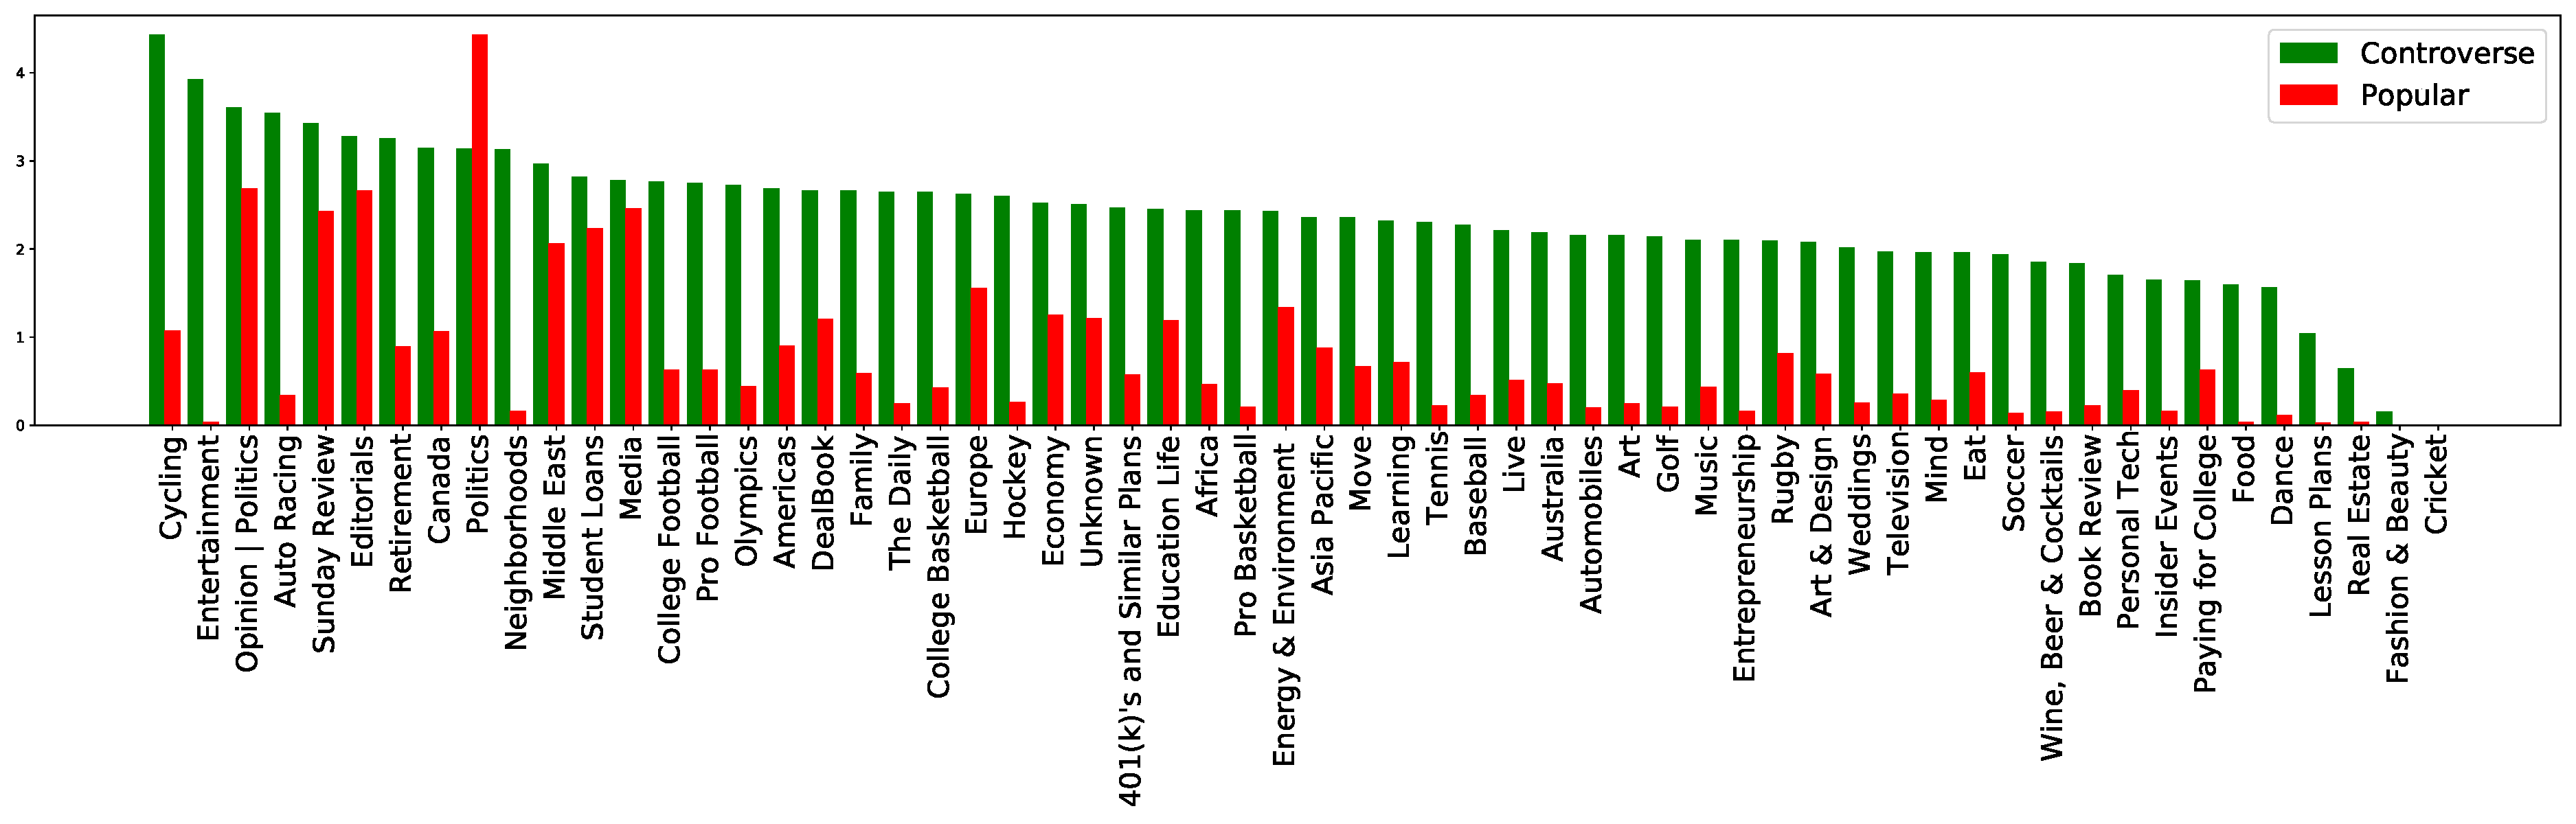
\includegraphics[width=\tw]{Pictures/Strat2SN.pdf}
\caption{Most controversial sections for Strategy 2}
\label{RG2}
\end{figure}

\begin{figure}
\centering
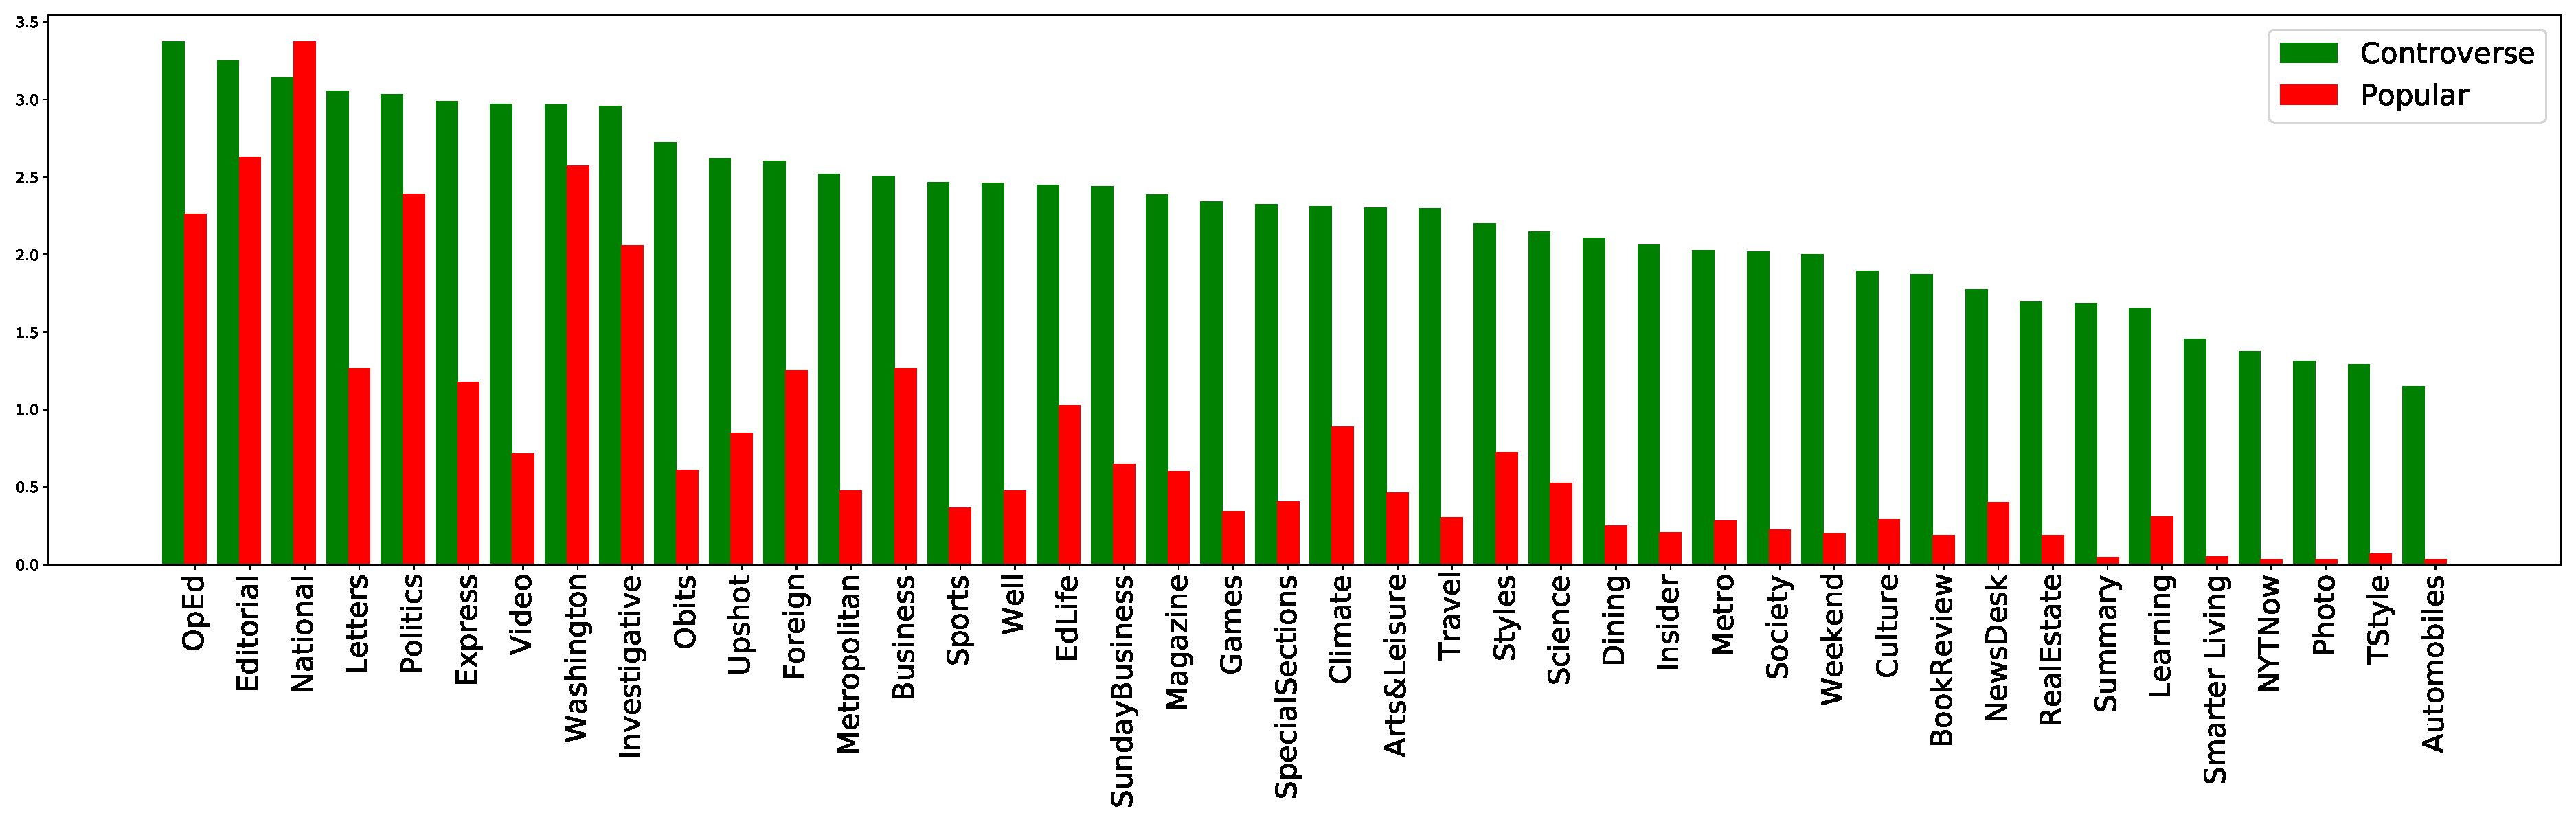
\includegraphics[width=\tw]{Pictures/Strat2ND.pdf}
\caption{Most controversial desks for Strategy 2}
\label{RG2nd}
\end{figure}

If we look at the averages on categories (FIg. \ref{RG2} and \ref{RG2nd}), it can be seen that popularity and controversy are now two very different quantities. The bar plots both for section name and desk show different behaviour between the two data series. However, the problem with Strategy 2 is that the categories labelled as "highly controversial" are quite unexpected, such as Cycling and Entertainment. On the other hand, controversial categories in Strategy 1 were Politics, Editorials and Middle East (categories one would expect to be controversial).


\begin{figure}
\centering
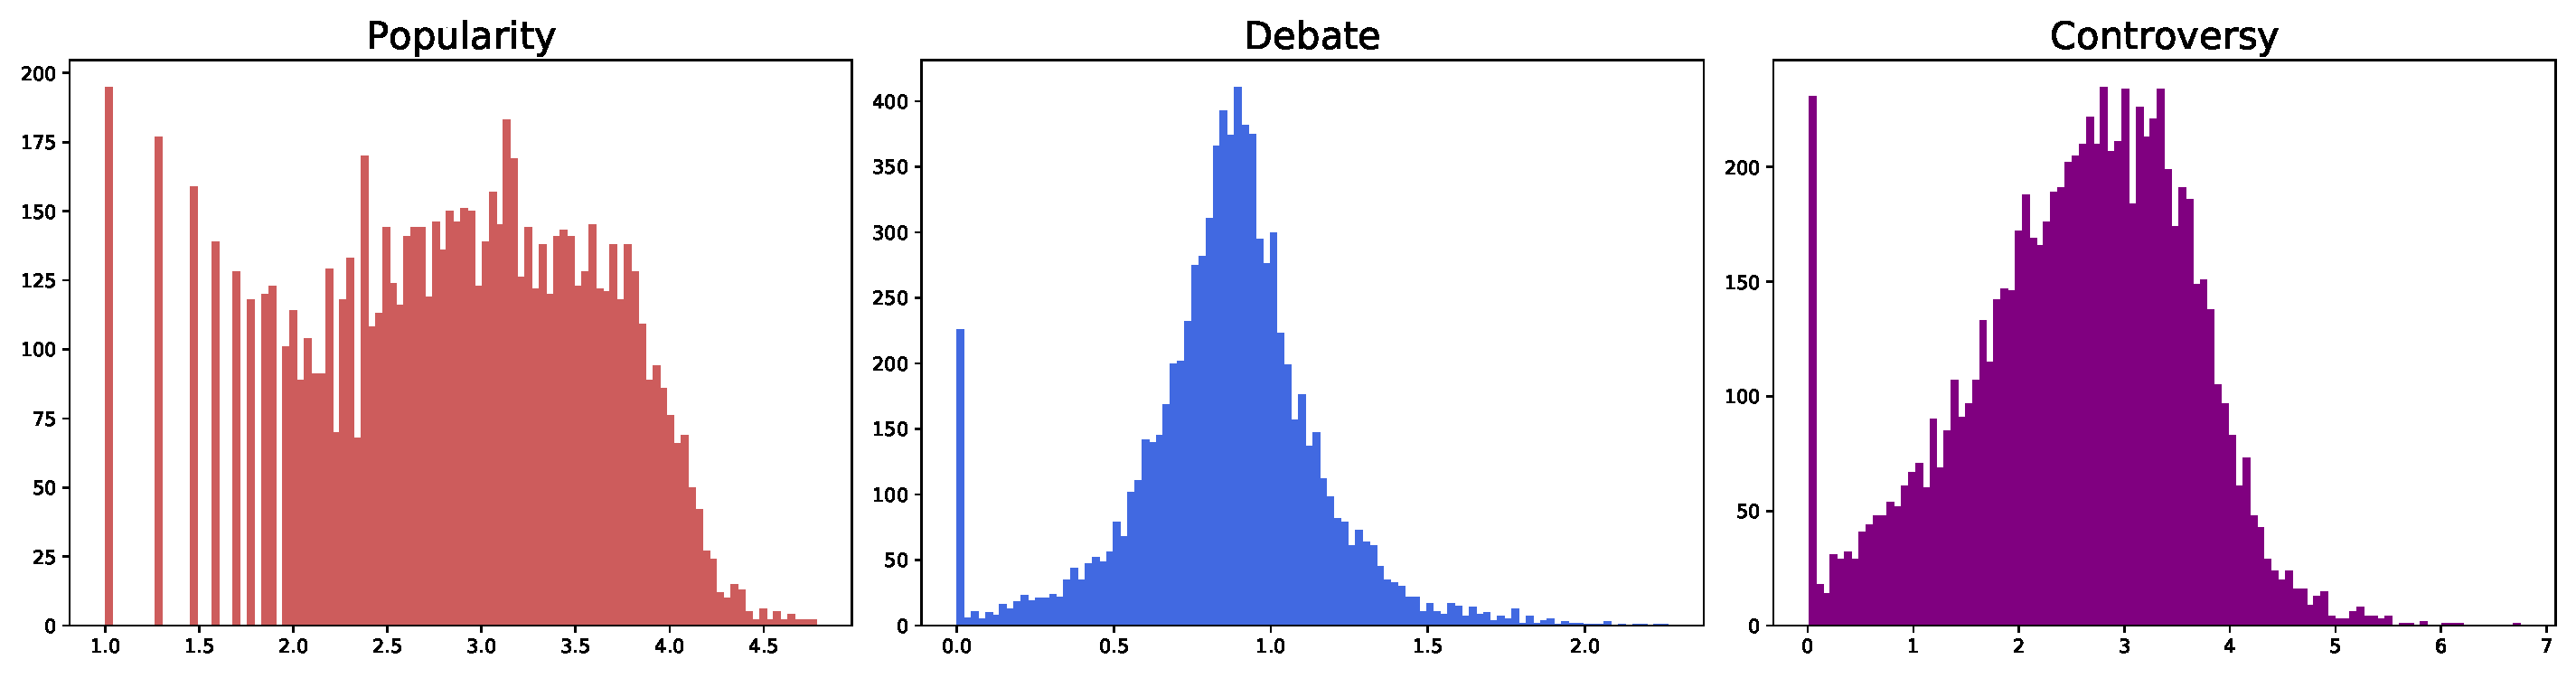
\includegraphics[width=\tw]{Pictures/Strat2Dist.pdf}
\caption{Popularity, Debate and Controversy distributions for Strategy 2.}
\label{Str1Dist}
\end{figure}


\begin{figure}[tb]
\centering
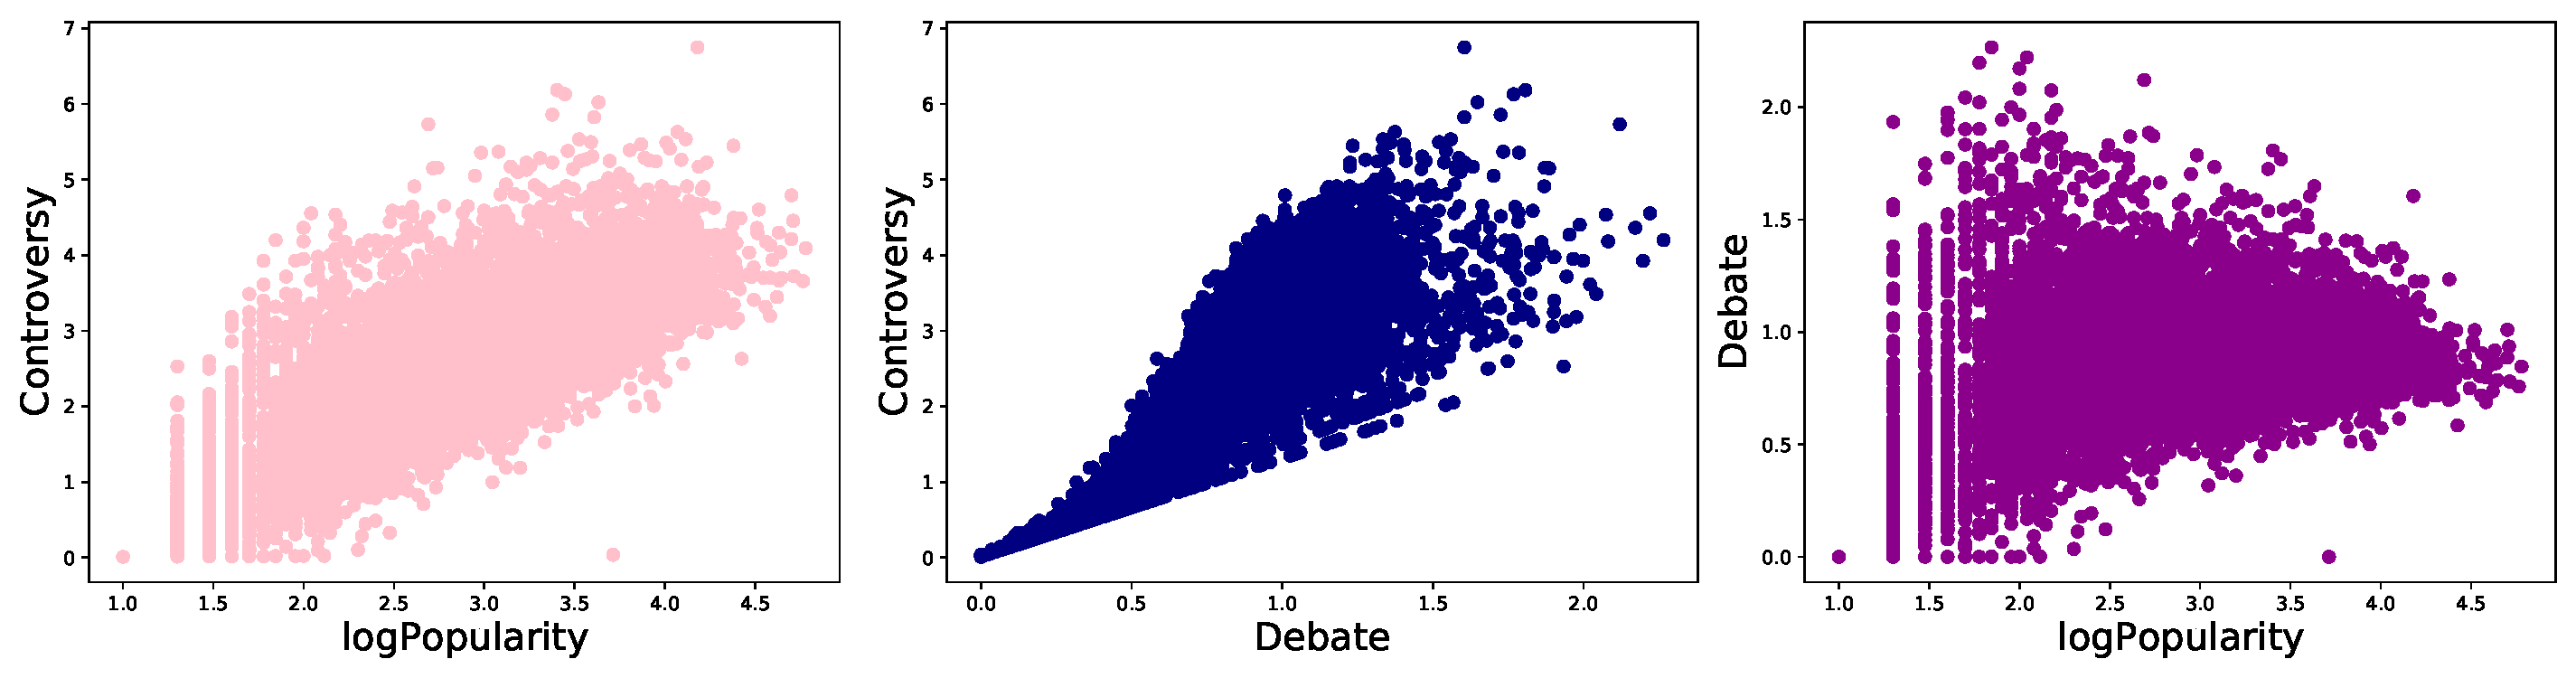
\includegraphics[width=\tw]{Pictures/Strat2Corr.pdf}
\caption{Correlation plots for Strategy 2.}
\label{Str1Corr}
\end{figure}


\subsection{Keyword extraction}
Lastly, a feature extraction was performed to check which words were common in comments related to the most controversial articles (top 10\%). A corpus vectorisation was performed via a {\tt TfidfVectorizer}, and then a $\chi2$ analysis was invoked to select words with higher score. Since TF-IDF tends to boost the score of words which are very uncommon in the corpus, among the "top controversial words" there were many nonsensical words, probably originated by typos of the comment authors. For this reason, only the words with a match in the AFINN dictionary were kept. Figure \ref{TopWords} depicts the words selected by the $\chi^2$ analysis.

\begin{figure}
\centering
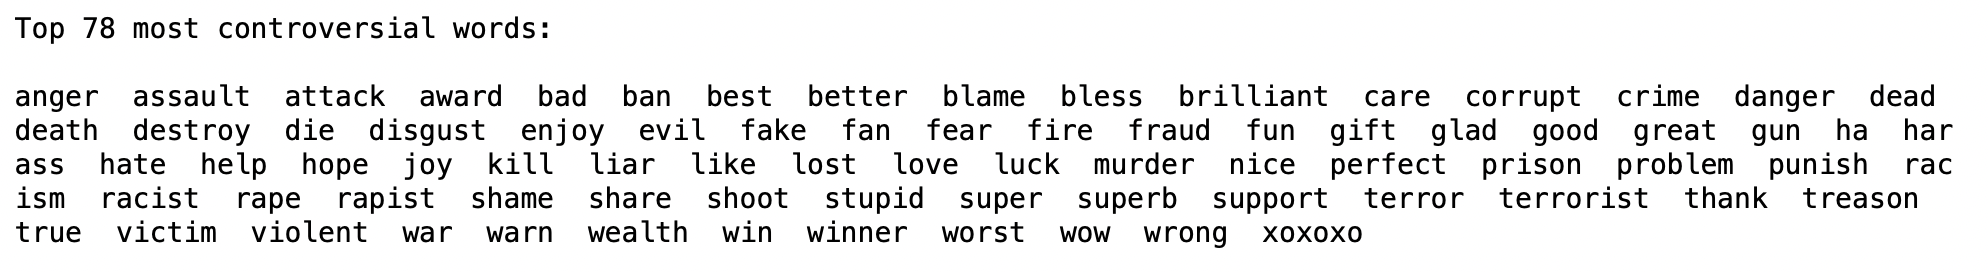
\includegraphics[width=\tw]{Pictures/TopWs.png}
\end{figure}